\documentclass[laboratorio]{guia}

\def \practnum {4} 
\def \practica {Ley de Inducci\'{o}n de Faraday}

\def \materia {Laboratorio de F\'\i sica II para Qu\'\i micos}
\def \periodo {2do. Cuatrimestre de 2015}
\def \catedra {Pablo Cobelli}
\def \website {http://materias.df.uba.ar/f2qa2015c2}
 
\usepackage{graphics}
\usepackage{amsmath}
\usepackage{amsfonts}
\usepackage{graphicx}
\usepackage{float}
\usepackage{wrapfig}
\usepackage{subfigure}
\usepackage{bm}
\usepackage{grffile}
\usepackage{color}
\usepackage{framed}
\usepackage[utf8]{inputenc}
\usepackage[T1]{fontenc}
\usepackage{lmodern}
\usepackage{circuitikz}
\usepackage[spanish]{babel}
\usepackage{babelbib}
\selectbiblanguage{spanish}

 

%----------------------------------------------------------
% Agrega al path de figuras el subdirectorio con el mismo
%     nombre que el archivo principal del proyecto
\graphicspath{{./\jobname/}}

%----------------------------------------------------------
% Definicion del entorno 'sabermas'
\makeatletter
\definecolor{shadecolor}{rgb}{0.89,0.91,0.94}
\newenvironment{sabermas}[1]{%
\vfill
\begin{shaded}
  \begin{center}
  {\textsection{Para saber m\'as}}
  \end{center}
  #1
\sf } 
{%
\end{shaded}%
}
\makeatother

%----------------------------------------------------------
% Definicion del entorno 'problema'
\newcounter{ContadorProblema}
\setcounter{ContadorProblema}{0}
\newcounter{TieneFiguraAsociada}
\setcounter{TieneFiguraAsociada}{0}
\newcounter{UbicacionFigura}
\setcounter{UbicacionFigura}{0}

\newenvironment{problema}[2][]
{%
    \ifx\relax#1\relax%
        \setcounter{TieneFiguraAsociada}{0}
        \else
        \setcounter{TieneFiguraAsociada}{1}
    \fi
    \def \archivofigura {#1}
    % 
    \refstepcounter{ContadorProblema}
    \noindent%
    \ifnum\value{TieneFiguraAsociada} < 1%
        {\sffamily \bfseries Problema \arabic{ContadorProblema}.}
        %{\sc {#1}}%
        \par\nobreak\par\nobreak%
        \medskip 
    \else
        % Va con figura; resta determinar de que lado.
        \ifnum\value{UbicacionFigura} < 1
            % Poner la figura del lado derecho
            \begin{minipage}{12.25cm}
            {\sffamily \bfseries Problema \arabic{ContadorProblema}.}
            %{\sc {#1}}%
            \par\nobreak\par\nobreak%
            \medskip 
        \else
            % Poner la figura del lado izquierdo
            \begin{minipage}{4.5cm}
                \centering
                \includegraphics[width=4.5cm]{\archivofigura}
                {\footnotesize {\sffamily Esquema asociado al 
                problema \arabic{ContadorProblema}}.}
            \end{minipage}\hfill%
            \begin{minipage}{12.25cm}
                {\sffamily \bfseries Problema \arabic{ContadorProblema}.}
                %{\sc {#1}}%
                \par\nobreak\par\nobreak%
                \medskip 
        \fi
    \fi
}
{%
    \ifnum\value{TieneFiguraAsociada} < 1%
        % \par \bigskip \vskip 0.3cm
    \else
        % Va con figura; resta determinar de que lado.
        \ifnum\value{UbicacionFigura} < 1
            % Poner la figura del lado derecho
            \end{minipage}\hfill%
            \begin{minipage}{4.5cm}
                \centering
                \includegraphics[width=4.5cm]{\archivofigura}
                {\footnotesize {\sffamily Esquema asociado al 
                problema \arabic{ContadorProblema}}.}
            \end{minipage}
        \else
            % Poner la figura del lado izquierdo
            \end{minipage}%
        \fi
    \fi
    \setcounter{TieneFiguraAsociada}{0}
    \par \bigskip \vskip 0.3cm
    % Permutamos el valor de la ubicacion
    \ifnum\value{UbicacionFigura} < 1
        \setcounter{UbicacionFigura}{1}
    \else
        \setcounter{UbicacionFigura}{0}
    \fi
}

%----------------------------------------------------------
% Definicion/Redefinicion de estilos
\renewcommand{\vec}[1]{\ensuremath{\mathbf{#1}}}



\hyphenation{ coe-fi-cien-tes coe-fi-cien-te au-to-va-lor
              au-to-va-lo-res co-rres-pon-der pro-ble-ma 
              cual-quie-ra po-la-ri-za-cio-nes }

\graphicspath{{./Guia_Induccion/}}

\begin{document} 
\objetivo{%
    El objetivo de esta guía experimental consiste en medir la fuerza electromotriz inducida sobre un circuito empleando para ello un generador de funciones y un osciloscopio (o un sistema de adquisición de señales asistido por computadora).
    \tematicas{fuerza electromotriz, inducción, ley de Faraday.}} 
\maketitle

\section{Ley de inducción de Faraday}
Allí donde hubiere un campo magnético \(\va{B}(\va{r},t)\) cualquier superficie \(\Sigma (t)\) que este atraviese circunscribirá un flujo magnético
\begin{equation}
  \va{\Phi_B} (t)= \iint_{\Sigma(t)} \va{B}(\va{r},t) \cdot \dd A.
\end{equation}

Faraday descubrió que de producirse una variación del flujo con el tiempo si en el borde de tal superficie \(\partial \Sigma\) hay un conductor se genera en él una fuerza electromotriz
\begin{equation}
  \varepsilon= - \dv{\va{\Phi_B}}{t}.
\end{equation}
que moviliza portadores de carga de forma tal de generar una corriente eléctrica que, siguiendo la ley de Ampère, da lugar a otro \(\va{B}'(t)\) que se opone a la variación de \(\va{\Phi_B}\).

De habeer una discontinuidad en el conductor que permita tener dos terminales para medir una diferencia de potencial se registrará que esta es tal que \(\Delta V = \varepsilon\).



\section{Inducción entre una bobina y un imán permanente}
En esta primera parte se propone abordar y responder experimentalmente a la siguiente pregunta: ¿qué sucede cuando el campo magnético generado por un imán permanente varía dentro de una bobina, por ejemplo cuando uno acerca o mueve un imán? 

Para responder a este interrogante, conecte una bobina al osciloscopio y registre (en función del tiempo) la diferencia de potencial que se induce en la misma cuando se acerca un imán a su interior.
Estudie también como varía la fuerza electromotriz inducida \(\varepsilon\) de acuerdo a como se mueve el imán (rápida o lentamente). 

Para poder observar una señal temporalmente corta (por ejemplo la debida al movimiento repentino del imán), resulta conveniente usar la función de disparo único del osciloscopio.
Consulte a su docente acerca de como habilitar dicho modo de trabajo en el osciloscopio.


\section{Inducción entre dos bobinas}
El dispositivo experimental propuesto para esta parte se ilustra esquemáticamente en la figura \ref{fig:1}.
El mismo consiste de una bobina con un número $N_1$ de espiras; este elemento constituye el denominado {\it primario} del circuito.
Dicha bobina se conecta a un generador de funciones a través de una resistencia $R$ (de entre 50 y \SI{500}{\ohm}).
El propósito de incluir esta resistencia es doble.
En primer lugar limitar la corriente que circula por la bobina.
En general se debe evitar conectar cualquier fuente de tensión (en este caso, el generador de funciones) a elementos de poca impedancia (inferior a \SI{50}{\ohm}) como la bobina, ya que se puede arruinar la fuente o quemar el circuito que esta alimenta al hacerle circular mucha corriente.
El otro propósito de esta resistencia es el de permitir medir la corriente $I$ que circula por el circuito primario. 

\begin{figure}[t!]
    \centering
    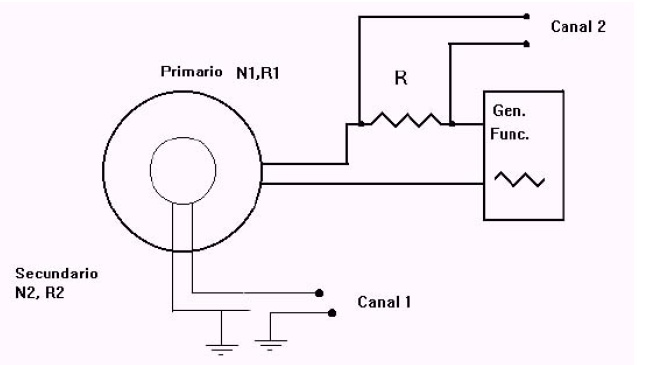
\includegraphics[width=8.5cm]{LG04--000.png}
    \caption{Esquema del dispositivo experimental propuesto para la segunda
    parte de la experiencia.}
    \label{fig:1}
\end{figure}

% A fin de realizar las mediciones, se propone el siguiente protocolo.
\subsection{Protocolo}
En un canal del osciloscopio se registra la caída de tensión $\Delta V_R$ en la resistencia, a partir de lo cual logramos obtener una señal que resulta proporcional a la \(I\).
Se debe tener en cuenta al diseñar el circuito que las tierras del generador de funciones y del osciloscopio deben coincidir (¿por qué?).
Una segunda bobina con un número de espiras $N_2$ se conecta al otro canal del osciloscopio; esta segunda bobina se denomina {\it el secundario} del presente dispositivo.

A continuación coloque una bobina dentro de la otra de modo tal que el campo magnético generado en el primario entre dentro del bobinado del secundario.
Aplique entonces una \(\Delta V\) sinusoidal al circuito de la figura \ref{fig:1}.
Estudie como varía la amplitud de \(\Delta V\) inducida en el secundario como función de la frecuencia del generador de funciones y luego en función de la amplitud de \(\Delta V\) del mismo.

Finalmente, se propone repetir la experiencia colocando ahora el núcleo de Fe en el interior de las bobinas.
Describa en forma cualitativa la relación entre las señales de \(I\) del primario y \(\Delta V\) del secundario.
Lleve a cabo esta experiencia con ondas sinusoidales y triangulares.
¿Porqué se puede decir que una señal es la derivada de la otra?


\section{Transformador}
Usando bobinas secundarias de diferente número de espiras, $N_2$, en los núcleos de Fe, pero manteniendo las condiciones del primario constantes (en amplitud y frecuencia), investigue la dependencia de $\Delta V_2$ en función de $N_2$. ¿Qué concluye? 

El dispositivo formado por dos bobinas o espiras que comparten sus flujos se conoce como {\it transformador}.
Mida y represente el cociente de amplitudes $\Delta V_2/\Delta V_1$ en función del cociente del número de espiras $N_2/N_1$.
Intente fabricar un transformador que duplique la tensión de línea y otro que la reduzca en un factor 3. 


\nocite{Alonso1998,Purcell1988,Reitz1996,Trelles1984,Reitz1996}
\bibliographystyle{unsrt} 
\bibliography{Bibliografia}

\end{document}
